\documentclass[12pt]{article}

\usepackage{amsmath,amssymb,amsfonts} %In case we need math stuff
\usepackage{graphicx} %For inserting images and stuff
\usepackage{listings} %For inserting code snippets
\usepackage{enumerate} %For fancy enumeration
\usepackage{pdfpages} %For adding the blockDiagram.pdf
\usepackage[margin=2cm]{geometry} %Nice margin setting
\graphicspath{ {C:/Users/Matthew/Downloads} }

\title{ECSE 321 - Intro to Software Engineering\\Software Architecture}
\author{Harley Wiltzer\\Camilo Garcia La Rotta\\Jake Shnaidman\\Robert Attard\\Matthew Lesko}
\date{February 19, 2017}

\begin{document}
\pagenumbering{gobble} %No page number on title page
\maketitle
\newpage
\pagenumbering{arabic} %Arabic numeral page numbers on regular pages
\tableofcontents
\section{Description}
	The software architecture comprises of two different patterns: a Model/View/Controller pattern
	and a Layered Architecture pattern. An "Authentication and Authorization" layer is on top of the
	MVC layer. Once the user is authenticated and authorized, they have access to the MVC layer. The
	MVC system contains three components which interact with each other: 
	\begin{itemize}
		\item Controller
		\item View
		\item Model
	\end{itemize}
	The Model component manages the system data and associated operations on that data; it
	encapsulates all the entities that are part of the model (can be seen in the model class
	diagram). The View component defines and manages how the data is presented to the user. The
	Controller component manages user interaction (key presses, mouse clicks, etc.) and passes these
	interactions to the View and the Model.
\section{Rationale}
	The MVC pattern was chosen because this allows the components to be changed independently. For
	example, adding a new view or changing an existing view can be done without any changes to the
	underlying data in the model. It allows the data to change independently of its representation
	and vice versa. It supports presentation of the same data in different ways with changes made in
	one representation shown in all of them. 
	The Layered Architecture pattern was used because the user would need to first authenticate
	him/herself and then receive authorization in order to interact with the sublayer.
\section{Block Diagram}
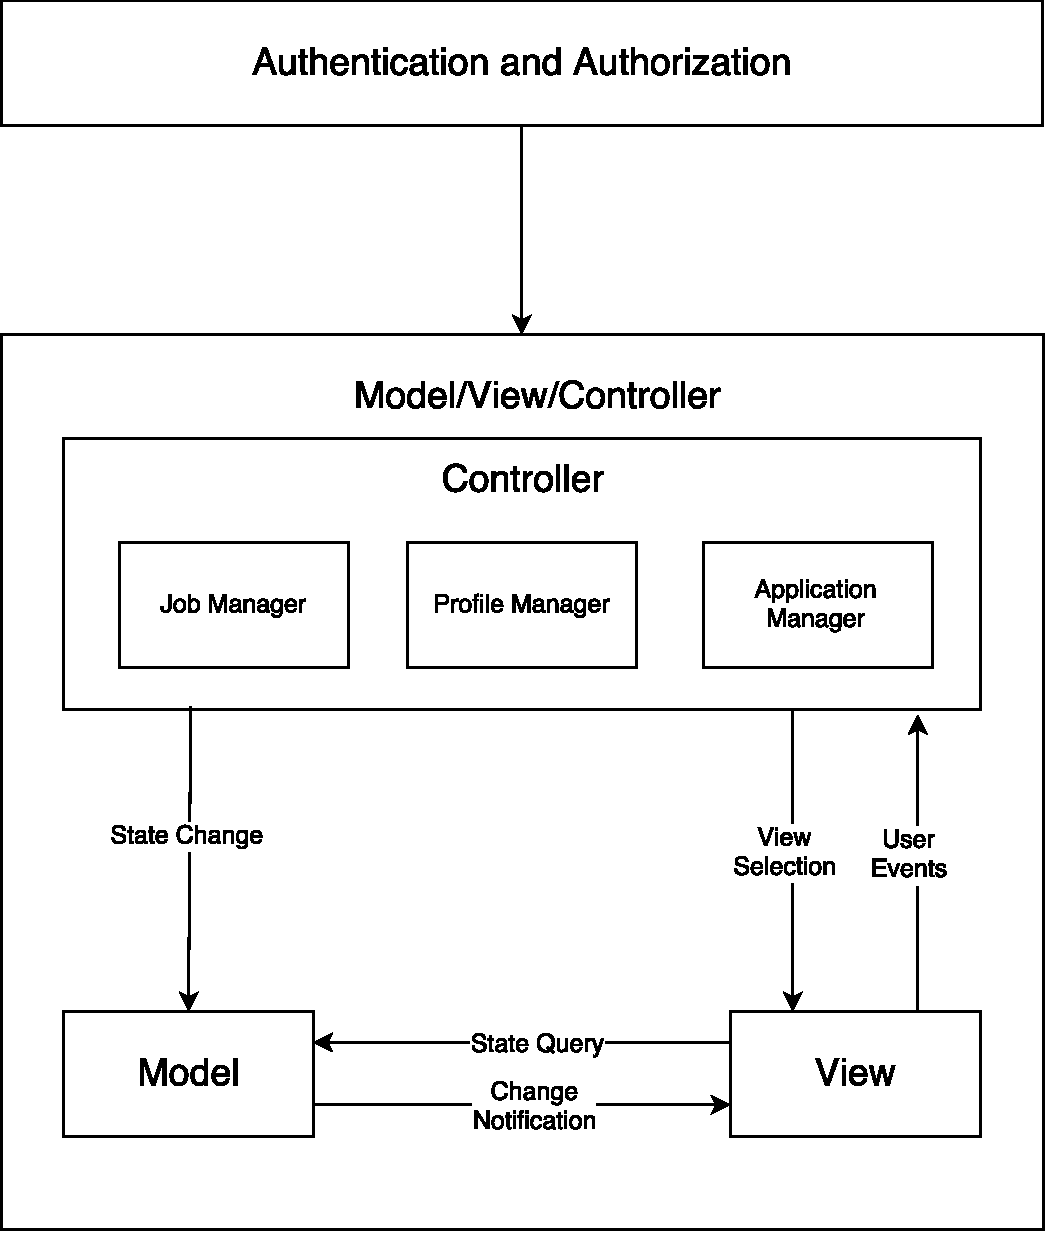
\includepdf[scale = 0.5, pages=1]{blockDiagram}
\end{document}
